\begin{figure}[H]
	\centering
	
	% First subfigure: Unit Impulse
	\begin{subfigure}{0.48\textwidth}
		\centering
		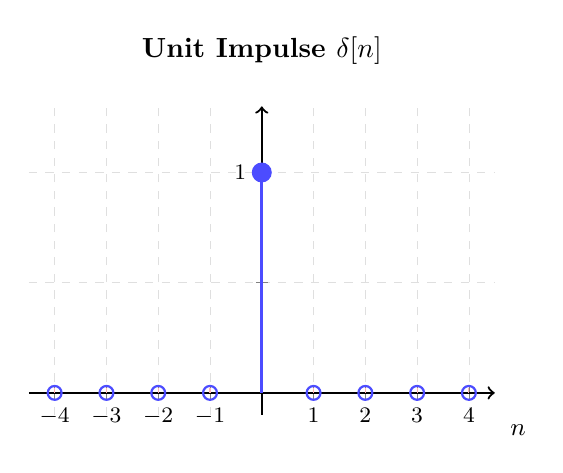
\begin{tikzpicture}
			\begin{axis}[
				width=7.5cm,
				height=5.5cm,
				axis lines=middle,
				xlabel={$n$},
				ylabel={},
				xmin=-4.5, 
				xmax=4.5,
				ymin=-0.1, 
				ymax=1.3,
				xtick={-4,-3,-2,-1,0,1,2,3,4},
				ytick={0,0.5,1},
				yticklabels={0,,1},
				grid=major,
				grid style={line width=0.2pt, draw=gray!25, dashed},
				font=\small,
				label style={font=\small},
				tick label style={font=\footnotesize},
				xlabel style={at={(axis description cs:1.05,0)}, anchor=north},
				ylabel style={at={(axis description cs:0,1.05)}, anchor=south},
				axis line style={->, thick},
				clip=false,
				title={Unit Impulse $\delta[n]$},
				title style={at={(0.5,1.05)}, font=\normalsize\bfseries}
				]
				% Plot the impulse at n=0 with stem
				\addplot[
				ycomb,
				very thick,
				color=blue!70,
				mark=*,
				mark size=3pt,
				mark options={fill=blue!70, draw=blue!70}
				] coordinates {(0,1)};
				% Add label for the impulse
				% Plot zeros with different style
				\addplot[
				only marks,
				mark=o,
				mark size=2.5pt,
				mark options={fill=blue, draw=blue!70, thick}
				] coordinates {(-4,0)(-3,0)(-2,0)(-1,0)(1,0)(2,0)(3,0)(4,0)};
				% Vertical lines for zeros (use \pgfplotsinvokeforeach)
				\pgfplotsinvokeforeach{-4,-3,-2,-1,1,2,3,4}{
					\draw[red!30, thin] (axis cs:#1,0) -- (axis cs:#1,0.02);
				}
			\end{axis}
		\end{tikzpicture}
		\caption{Unit Impulse}
	\end{subfigure}
	\hfill
	% Second subfigure: Unit Step
	\begin{subfigure}{0.48\textwidth}
		\centering
		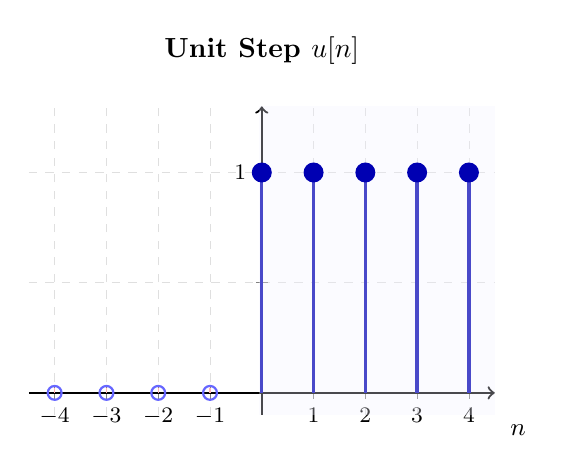
\begin{tikzpicture}
			\begin{axis}[
				width=7.5cm,
				height=5.5cm,
				axis lines=middle,
				xlabel={$n$},
				ylabel={},
				xmin=-4.5, 
				xmax=4.5,
				ymin=-0.1, 
				ymax=1.3,
				xtick={-4,-3,-2,-1,0,1,2,3,4},
				ytick={0,0.5,1},
				yticklabels={0,,1},
				grid=major,
				grid style={line width=0.2pt, draw=gray!25, dashed},
				font=\small,
				label style={font=\small},
				tick label style={font=\footnotesize},
				xlabel style={at={(axis description cs:1.05,0)}, anchor=north},
				ylabel style={at={(axis description cs:0,1.05)}, anchor=south},
				axis line style={->, thick},
				clip=false,
				title={Unit Step $u[n]$},
				title style={at={(0.5,1.05)}, font=\normalsize\bfseries}
				]
				% Plot ones (n >= 0) with stems
				\addplot[
				ycomb,
				very thick,
				color=blue!70!black,
				mark=*,
				mark size=3pt,
				mark options={fill=blue!70!black, draw=blue!70!black}
				] coordinates {(0,1)(1,1)(2,1)(3,1)(4,1)};
				% Labels for the ones
				% Plot zeros (n < 0)
				\addplot[
				only marks,
				mark=o,
				mark size=2.5pt,
				mark options={fill=blue, draw=blue!60, thick}
				] coordinates {(-4,0)(-3,0)(-2,0)(-1,0)};
				% Vertical lines for zeros
				\pgfplotsinvokeforeach{-4,-3,-2,-1}{
					\draw[red!30, thin] (axis cs:#1,0) -- (axis cs:#1,0.02);
				}
				% Background shading for n >= 0 region
				\fill[blue!5, opacity=0.3] (axis cs:-0.05,-0.1) rectangle (axis cs:4.5,1.3);
			\end{axis}
		\end{tikzpicture}
		\caption{Unit Step}
	\end{subfigure}

	\label{fig:discrete_signals}
\end{figure}
